\chapter{Results Description}
\label{chap:results}
\begin{chapterintro}
In this chapter we will make a deep insight on the data obtained from the \emph{Data Mining} process described in chapter~\ref{chap:datamining}.

We will analyse the resultsets from different points of view. Using the evaluation parameters already defined, we will provide further details on the actual use these resultsets can have for maintenance operators according to their performance. Differences between different maintenance stations and time periods will as well be analysed.

To finish, we will present an example scenario in which we will be able to understand the actual effect our results would have on daily maintenance operations.
\end{chapterintro}
\section{Description of obtained rulesets}
\label{sec:desc_results}
The result of the previous work described in section~\ref{sec:assoc_rules} comes in the form of a set of association rules. These \emph{rule sets} contain a list of all the association rules found, along with their performance value calculed by the \emph{K-fold-CV} procedure as defined in section~\ref{sec:validation_evaluation}. The obtained rulesets and the number of rules they contain can be seen in table~\ref{tab:numrules}. Our goal was to generate different rulesets for each of our maintenance stations, each of them covering different time windows. Specifically, we have studied three different time windows: one day, two days and one week. This defines the observation period for our predictive work, which means not only the time span we will use as antecedents for our rules but also the time window within which our prediction can occur.

These sets contain all the information obtained from the procedure defined in section~\ref{sec:assoc_rules}. It is important to note that not all of them will be useful in order to implement a predictive system, as their precision is sometimes as low as 5\%. The threshold for a rule to be useful needs to be defined by maintenance workers who know the associated costs of maintenance tasks required to handle raised predictions before knowing if they will actually happen. If some event needs a significantly high amount of money to be avoided we will probably want to be \emph{very} confident about our precisions regarding that kind of event before investing resources on preventing it.

However, in general terms we can consider a prediction is good when it has more chances of being a right guess than a wrong one. We will therefore set p=0.5 as the point where rules \emph{start} to be useful. Rules with lower precisions are still provided and can be useful for other analysis tasks or further research, but from now on we will disregard them and focus on the \emph{0.5 set} which can be used right away for predictive purposes. These new sets and their size can be seen in table~\ref{tab:numrules_50}. Obviously, the size of the sets reduces drastically when imposing this kind of conditions.

\begin{table}
\begin{center}
\begin{tabular}{|c|c|c|}
\hline \headcell{Station} & \headcell{Time Window} & \headcell{Rules} \\ 
\hline 
Station A & 1 day & 27522 \\ 
\hline 
Station A & 7 days & 50281 \\ 
\hline 
Station B & 1 day & 39214 \\ 
\hline 
Station C & 1 day & 113 \\ 
\hline 
Station C & 2 days & 72 \\ 
\hline
Station C & 7 days & 133 \\ 
\hline 
Station D & 1 day & 8091 \\ 
\hline 

\end{tabular} 
\caption{Size of obtained rule sets for each station and time window} \label{tab:numrules}
\end{center}
\end{table}

\begin{table}
\begin{center}
\begin{tabular}{|c|c|c|}
\hline \headcell{Station} & \headcell{Time Window} & \headcell{Rules} \\ 
\hline 
Station A & 7 days & 9 \\ 
\hline 
Station B & 1 day & 7104 \\ 
\hline 
Station C & 1 day & 31 \\ 
\hline 
Station C & 2 days & 30 \\ 
\hline
Station C & 7 days & 48 \\ 
\hline 
Station D & 1 day & 242 \\ 
\hline 

\end{tabular} 
\caption{Number of rules for each set setting a threshold of 50\% precision} \label{tab:numrules_50}
\end{center}
\end{table}



At this point, it is important to remember the decisions taken in terms of search depth and data subsetting as mentioned in sections~\ref{sec:search_parameters} and~\ref{sec:dataclustering}. In these terms, rule sets for some of the stations and time windows could not be generated with our available computation capabilities. A better server or algorithm optimisation would be required in order to obtain result sets for these cases.

\subsection{Number of rules against precision}
\label{sec:rules_vs_prec}
As we have seen in section~\ref{sec:desc_results}, the amount of rules decreases significantly if we impose strict conditions for their validity. In this section we will perform a deeper analysis on how amount of rules vary when setting different thresholds. For this purpose, we will set different thresholds and check the number of rules complying with this condition. The results are shown in tables \ref{tab:numrules_thresh_albacete7}, \ref{tab:numrules_thresh_antequera1}, \ref{tab:numrules_thresh_segovia1}, \ref{tab:numrules_thresh_segovia2}, \ref{tab:numrules_thresh_segovia7} and \ref{tab:numrules_thresh_sevilla1}. As expected, the number of rules increases exponentially when decreasing the threshold. For better visualization, these amounts for the \emph{$>50\%$ subsets} are represented in figures~\ref{fig:precision_alb7}, \ref{fig:precision_ant1}, \ref{fig:precision_seg1}, \ref{fig:precision_seg2}, \ref{fig:precision_seg7} and \ref{fig:precision_sev1}.

\begin{table}
\begin{center}
\begin{tabular}{|c|c|c|}
\hline \headcell{Threshold} & \headcell{Number of rules} \\ 
\hline 
0.05 & 44620 \\ 
\hline 
0.10 & 38007 \\ 
\hline 
0.20 & 4060 \\ 
\hline 
0.30 & 30 \\ 
\hline
0.40 & 27 \\ 
\hline 
0.50 & 9 \\ 
\hline 
0.60 & 8 \\ 
\hline 

\end{tabular} 
\caption{Number of rules for different thresholds in Station A (7 days)} \label{tab:numrules_thresh_albacete7}
\end{center}
\end{table}

\begin{table}
\begin{center}
\begin{tabular}{|c|c|c|}
\hline \headcell{Threshold} & \headcell{Number of rules} \\ 
\hline 
0.05 & 31846 \\ 
\hline 
0.10 & 28338 \\ 
\hline 
0.20 & 21566 \\ 
\hline 
0.30 & 15829 \\ 
\hline
0.40 & 10876 \\ 
\hline 
0.50 & 7137 \\ 
\hline 
0.60 & 4928 \\ 
\hline 
0.70 & 891 \\ 
\hline 
0.80 & 47 \\ 
\hline 

\end{tabular} 
\caption{Number of rules for different thresholds in Station B (1 day)} \label{tab:numrules_thresh_antequera1}
\end{center}
\end{table}

\begin{table}
\begin{center}
\begin{tabular}{|c|c|c|}
\hline \headcell{Threshold} & \headcell{Number of rules} \\ 
\hline 
0.05 & 106 \\ 
\hline 
0.10 & 95 \\ 
\hline 
0.20 & 72 \\ 
\hline 
0.30 & 44 \\ 
\hline
0.40 & 33 \\ 
\hline 
0.50 & 31 \\ 
\hline 
0.60 & 30 \\ 
\hline 
0.70 & 24 \\ 
\hline 
0.80 & 12 \\ 
\hline 

\end{tabular} 
\caption{Number of rules for different thresholds in Station C (1 day)} \label{tab:numrules_thresh_segovia1}
\end{center}
\end{table}

\begin{table}
\begin{center}
\begin{tabular}{|c|c|c|}
\hline \headcell{Threshold} & \headcell{Number of rules} \\ 
\hline 
0.05 & 69 \\ 
\hline 
0.10 & 66 \\ 
\hline 
0.20 & 56 \\ 
\hline 
0.30 & 40 \\ 
\hline
0.40 & 31 \\ 
\hline 
0.50 & 30 \\ 
\hline 
0.60 & 14 \\ 
\hline 

\end{tabular} 
\caption{Number of rules for different thresholds in Station C (2 days)} \label{tab:numrules_thresh_segovia2}
\end{center}
\end{table}

\begin{table}
\begin{center}
\begin{tabular}{|c|c|c|}
\hline \headcell{Threshold} & \headcell{Number of rules} \\ 
\hline 
0.05 & 128 \\ 
\hline 
0.10 & 125 \\ 
\hline 
0.20 & 92 \\ 
\hline 
0.30 & 75 \\ 
\hline
0.40 & 64 \\ 
\hline 
0.50 & 48 \\ 
\hline 
0.60 & 35 \\ 
\hline 
0.70 & 30 \\ 
\hline 
0.80 & 25 \\ 
\hline 
0.90 & 4 \\ 
\hline 

\end{tabular} 
\caption{Number of rules for different thresholds in Station C (7 days)} \label{tab:numrules_thresh_segovia7}
\end{center}
\end{table}

\begin{table}
\begin{center}
\begin{tabular}{|c|c|c|}
\hline \headcell{Threshold} & \headcell{Number of rules} \\ 
\hline 
0.05 & 6730 \\ 
\hline 
0.10 & 2832 \\ 
\hline 
0.20 & 2357 \\ 
\hline 
0.30 & 1799 \\ 
\hline
0.40 & 642 \\ 
\hline 
0.50 & 246 \\ 
\hline 
0.60 & 78 \\ 
\hline 
0.70 & 2 \\ 
\hline 

\end{tabular} 
\caption{Number of rules for different thresholds in Station D (1 day)} \label{tab:numrules_thresh_sevilla1}
\end{center}
\end{table}

\begin{figure}[hbtp]
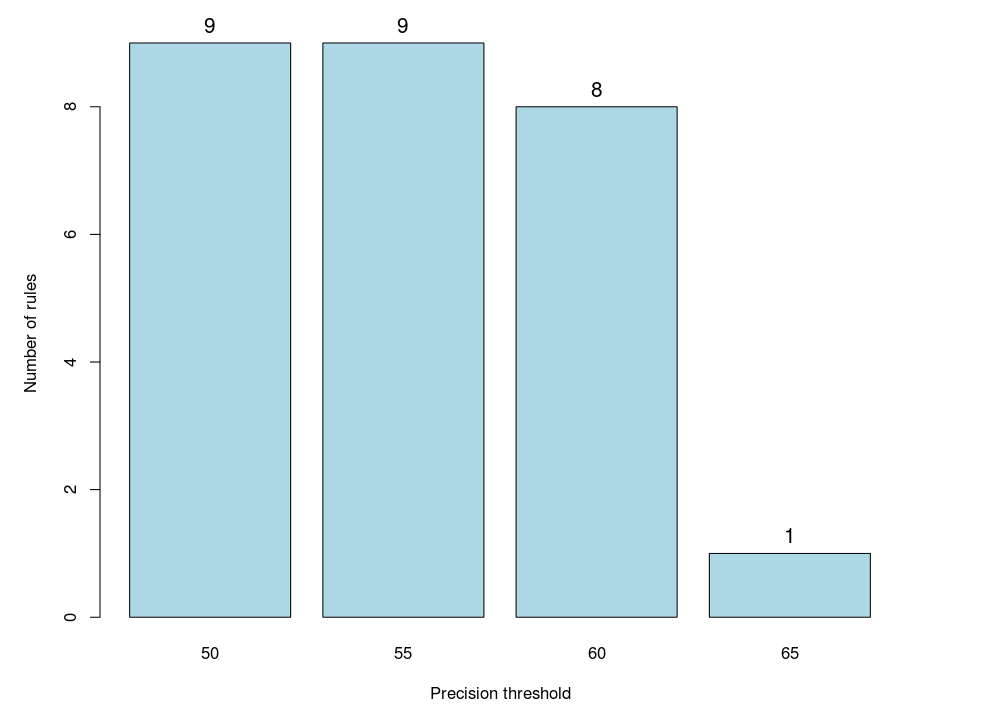
\includegraphics[width=\textwidth]{img/precision_alb7.png}
\caption{Number of rules for different thresholds in Station A (7 days)} \label{fig:precision_alb7}
\end{figure}

\begin{figure}[hbtp]
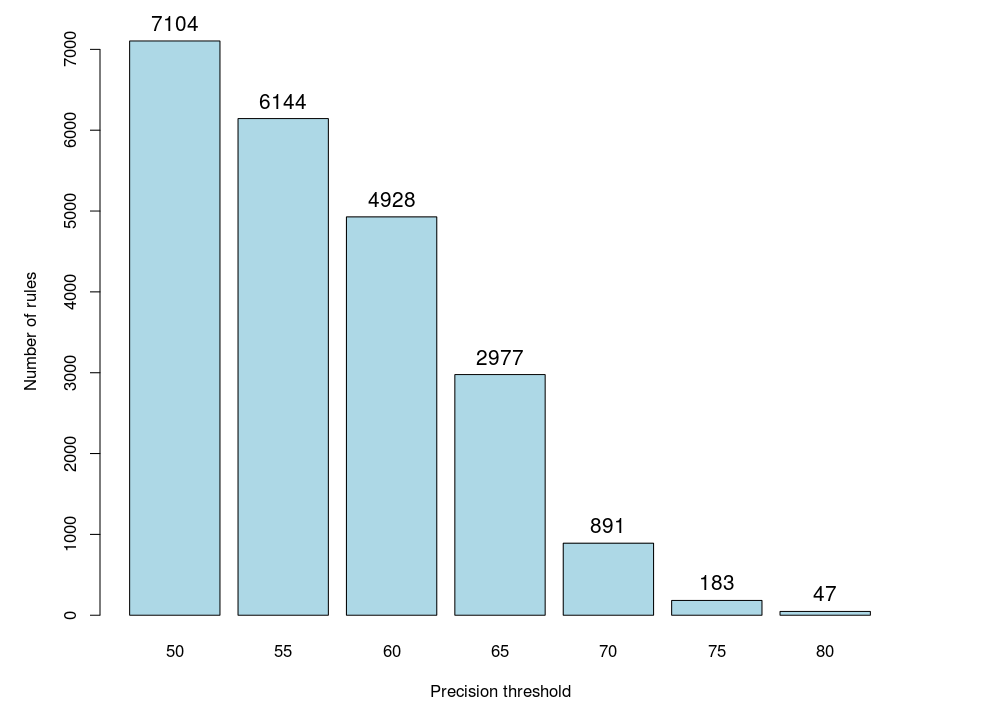
\includegraphics[width=\textwidth]{img/precision_ant1.png}
\caption{Number of rules for different thresholds in Station B (1 day)} \label{fig:precision_ant1}
\end{figure}

\begin{figure}[hbtp]
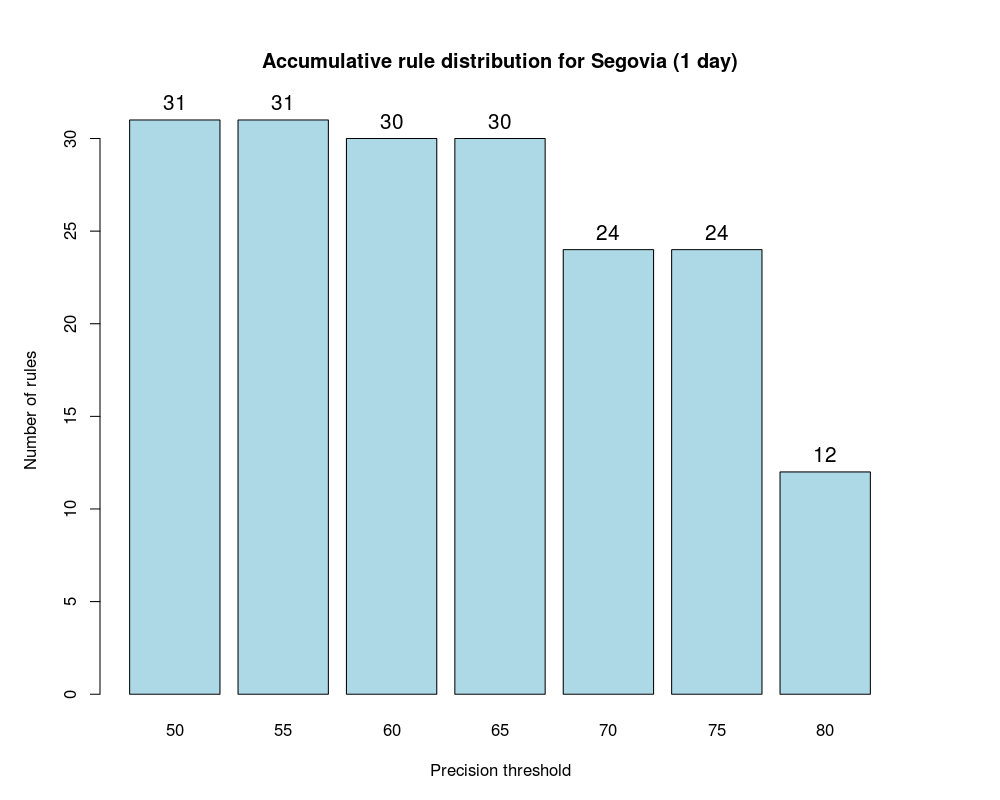
\includegraphics[width=\textwidth]{img/precision_seg1.png}
\caption{Number of rules for different thresholds in Station C (1 day)} \label{fig:precision_seg1}
\end{figure}

\begin{figure}[hbtp]
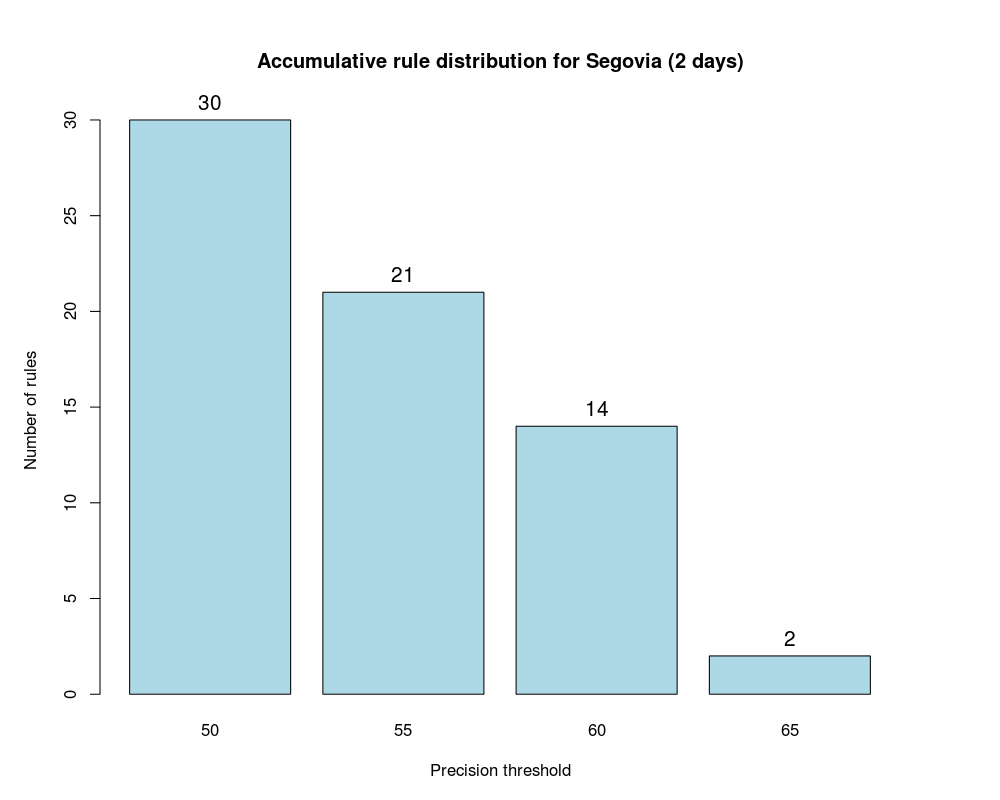
\includegraphics[width=\textwidth]{img/precision_seg2.png}
\caption{Number of rules for different thresholds in Station C (2 days)} \label{fig:precision_seg2}
\end{figure}

\begin{figure}[hbtp]
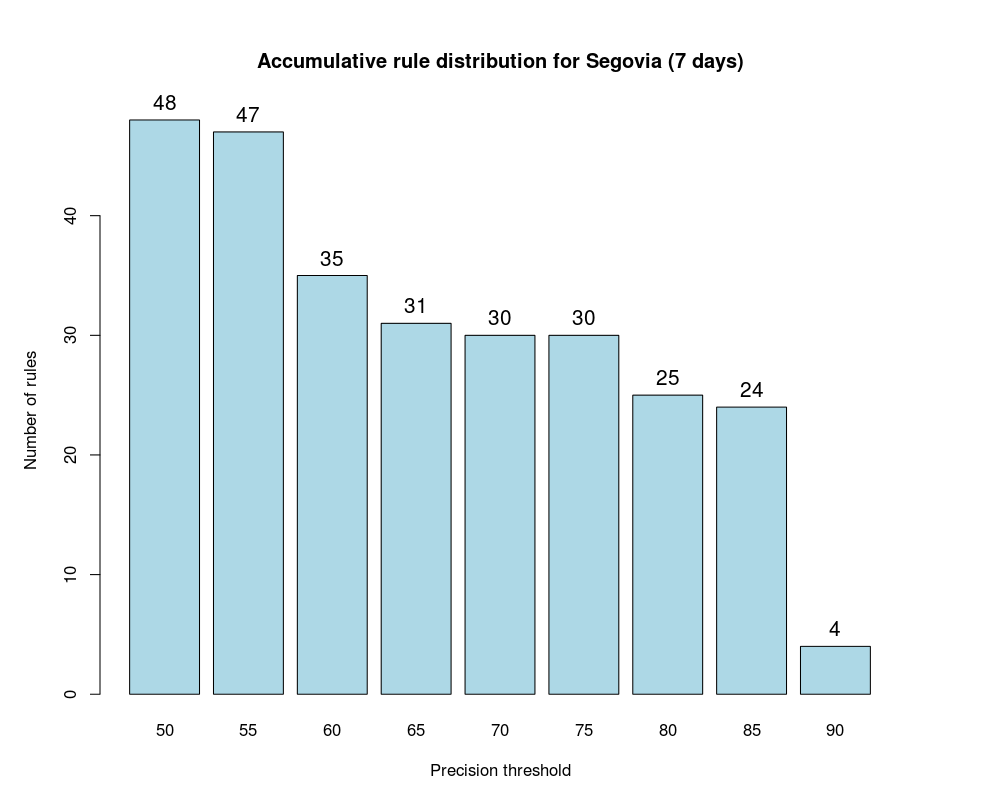
\includegraphics[width=\textwidth]{img/precision_seg7.png}
\caption{Number of rules for different thresholds in Station C (7 days)} \label{fig:precision_seg7}
\end{figure}

\begin{figure}[hbtp]
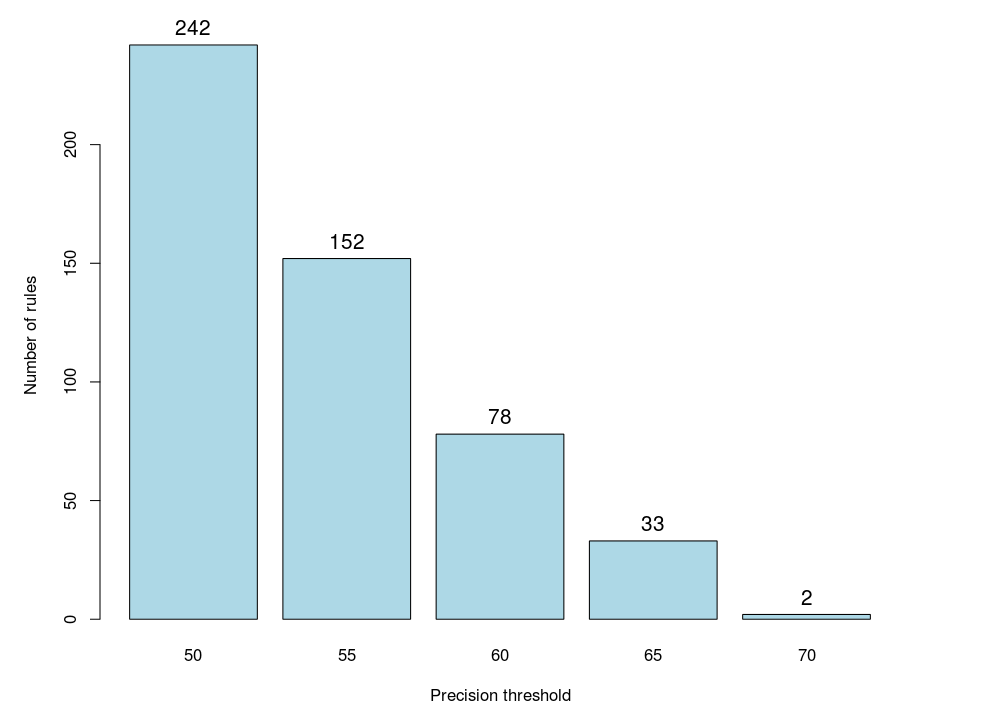
\includegraphics[width=\textwidth]{img/precision_sev1.png}
\caption{Number of rules for different thresholds in Station D (1 day)} \label{fig:precision_sev1}
\end{figure}

\clearpage

\subsection{Precision distribution}
\label{sec:precision_distribution}
In section~\ref{sec:rules_vs_prec} we analysed the number of rules we would obtain if we set different precision levels as thresholds to generate different subsets. According to our expectations, we observed a decay in these numbers as we set higher thresholds. However, this decay, although apparently exponential, shows flat zones and other irregularities which would be unexpected at first.

In order to better visualize these anomalities we will graphically represent the precision distribution in form of histograms for the previous sets. These distributions can be seen in figures~\ref{fig:hist_alb7}, \ref{fig:hist_ant1}, \ref{fig:hist_seg1}, \ref{fig:hist_seg2}, \ref{fig:hist_seg7} and \ref{fig:hist_sev1}.

In these histograms we can see that the distribution does not grow exponentially as we lower the precision, as we would expect and as we apparently saw in the analysis from section~\ref{sec:rules_vs_prec}. Instead, there are some accumulation points around which precision tends to take values. 

For example, looking at the distribution for Station B (figure~\ref{fig:hist_ant1}) we see that there are more rules with precisions between 0.65 and 0.70 than between 0.50 and 0.55.

As we do not have large sets of rules for all the stations, performing a deeper analysis of the distributions is not possible. As these kind of irregularities appear for all the studied cases, it is very unlikely that they are caused just by chance. However, the causes and possible implications of these distributions cannot be infered at this point and would require further research.

\begin{figure}[hbtp]
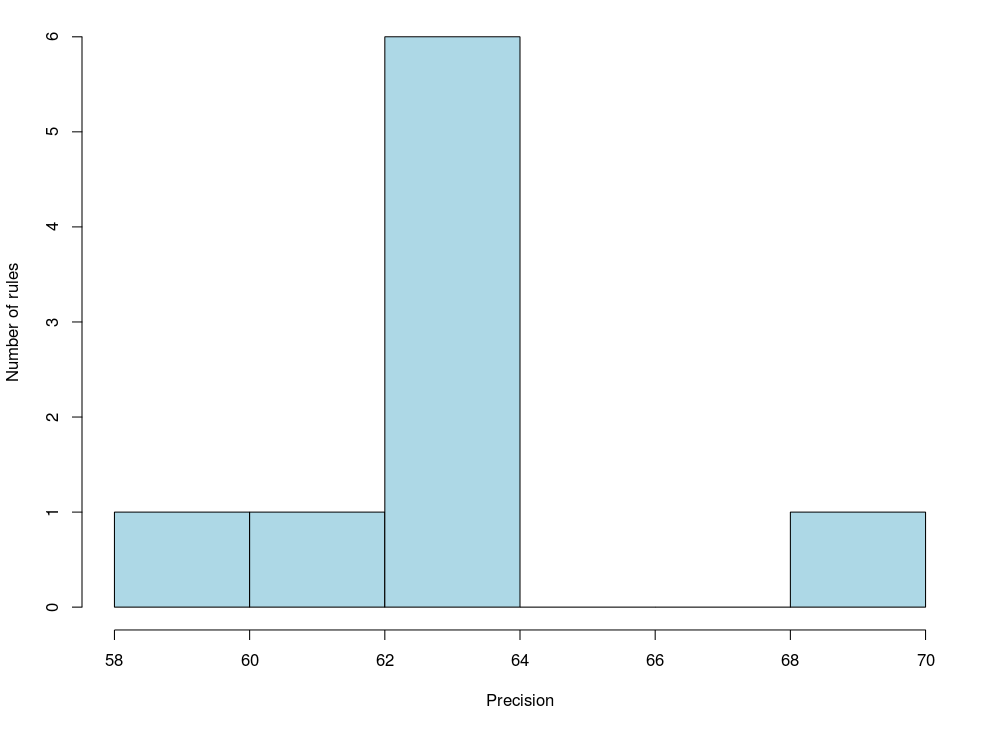
\includegraphics[width=\textwidth]{img/hist_alb7.png}
\caption{Rule distribution by precision in Station A (7 days)} \label{fig:hist_alb7}
\end{figure}

\begin{figure}[hbtp]
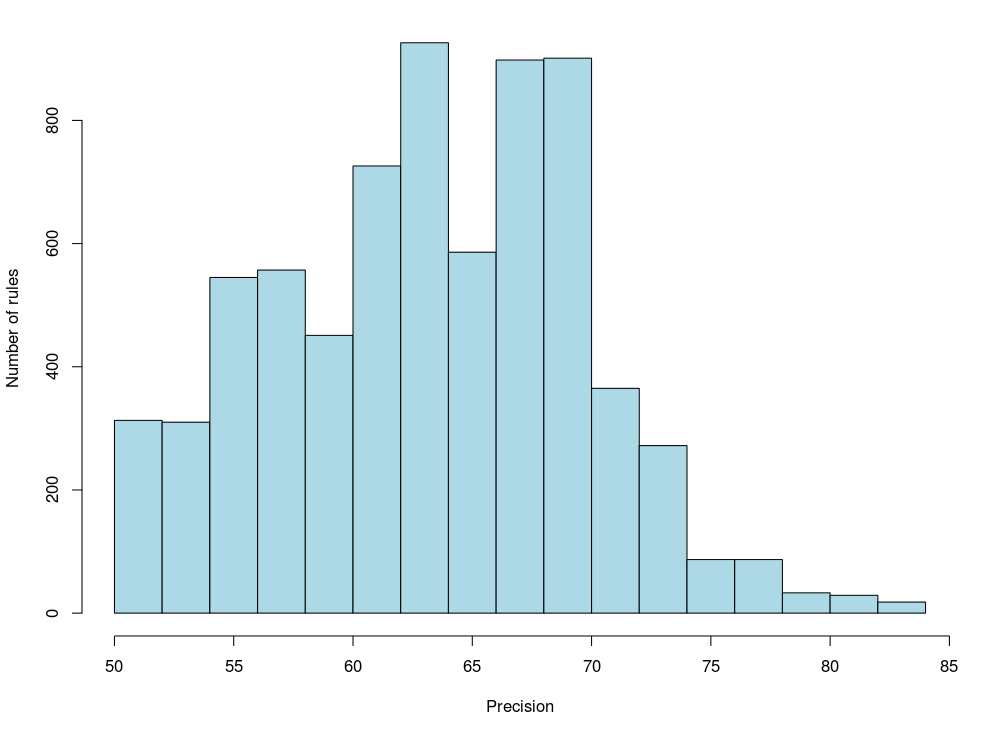
\includegraphics[width=\textwidth]{img/hist_ant1.png}
\caption{Rule distribution by precision in Station B (1 day)} \label{fig:hist_ant1}
\end{figure}

\begin{figure}[hbtp]
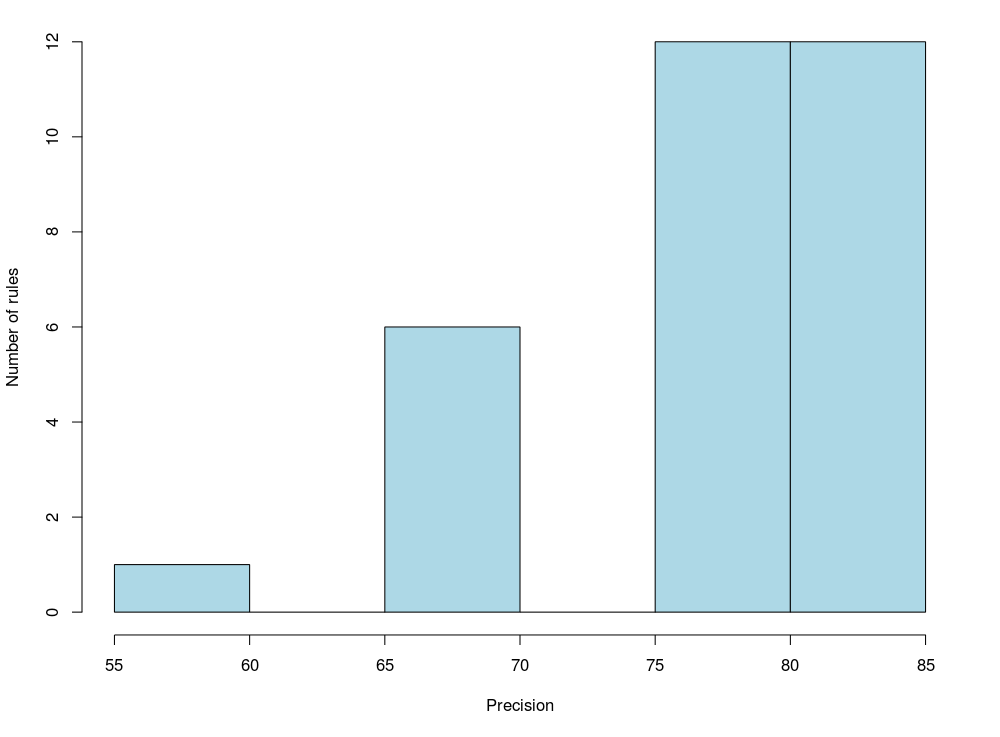
\includegraphics[width=\textwidth]{img/hist_seg1.png}
\caption{Rule distribution by precision in Station C (1 day)} \label{fig:hist_seg1}
\end{figure}

\begin{figure}[hbtp]
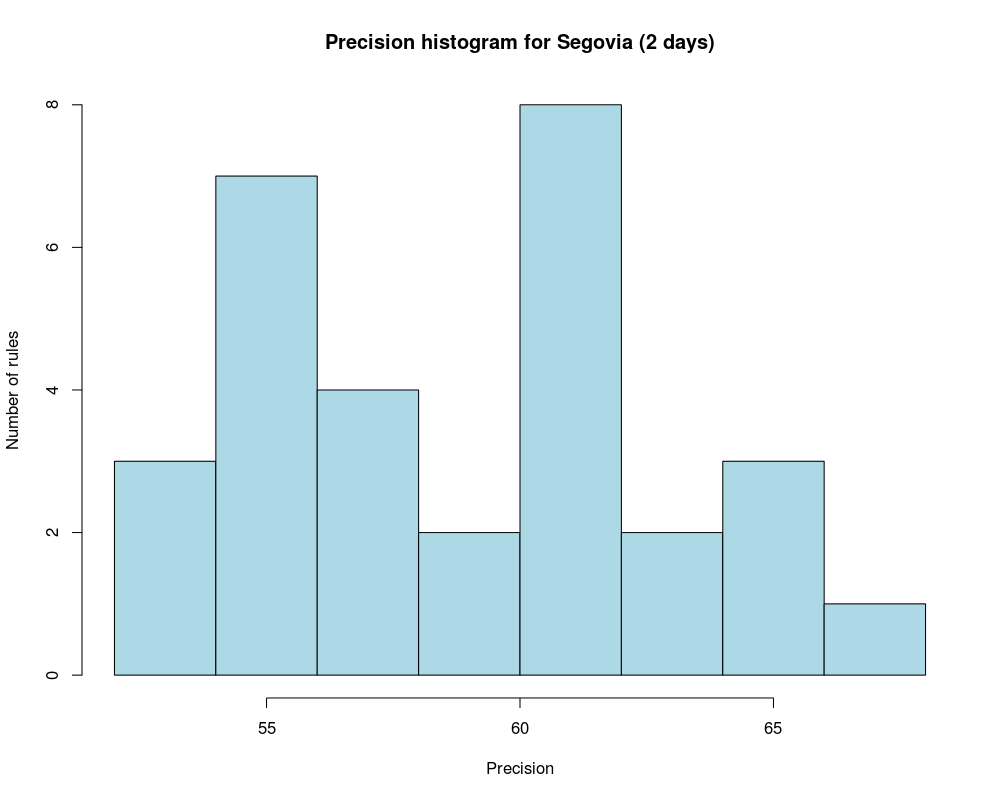
\includegraphics[width=\textwidth]{img/hist_seg2.png}
\caption{Rule distribution by precision in Station C (2 days)} \label{fig:hist_seg2}
\end{figure}

\begin{figure}[hbtp]
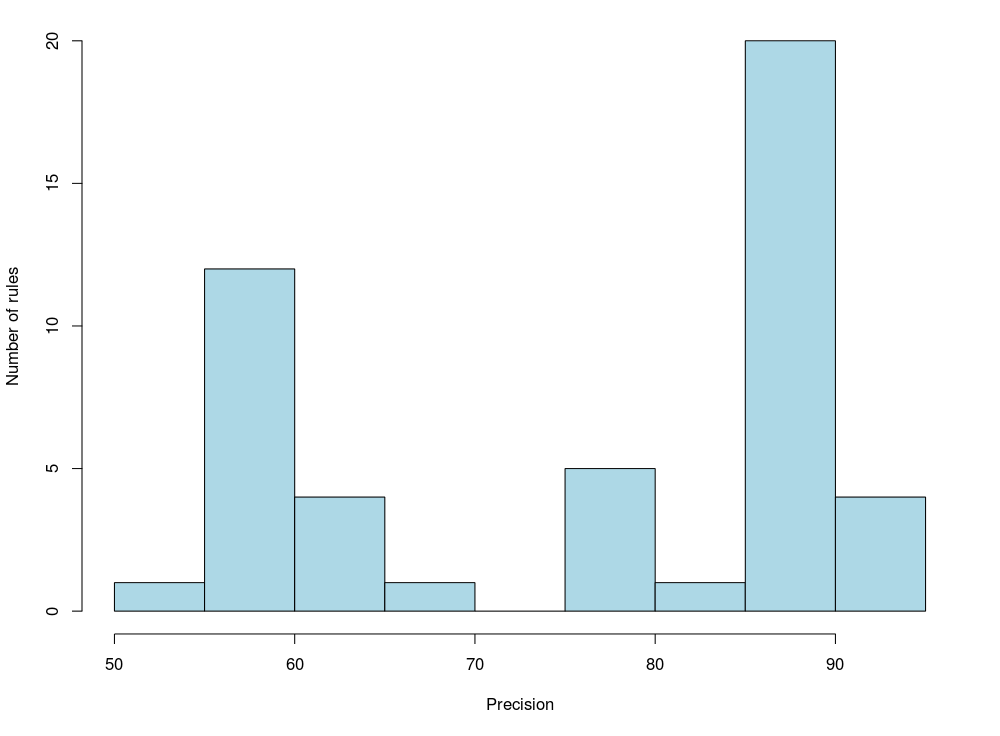
\includegraphics[width=\textwidth]{img/hist_seg7.png}
\caption{Rule distribution by precision in Station C (7 days)} \label{fig:hist_seg7}
\end{figure}

\begin{figure}[hbtp]
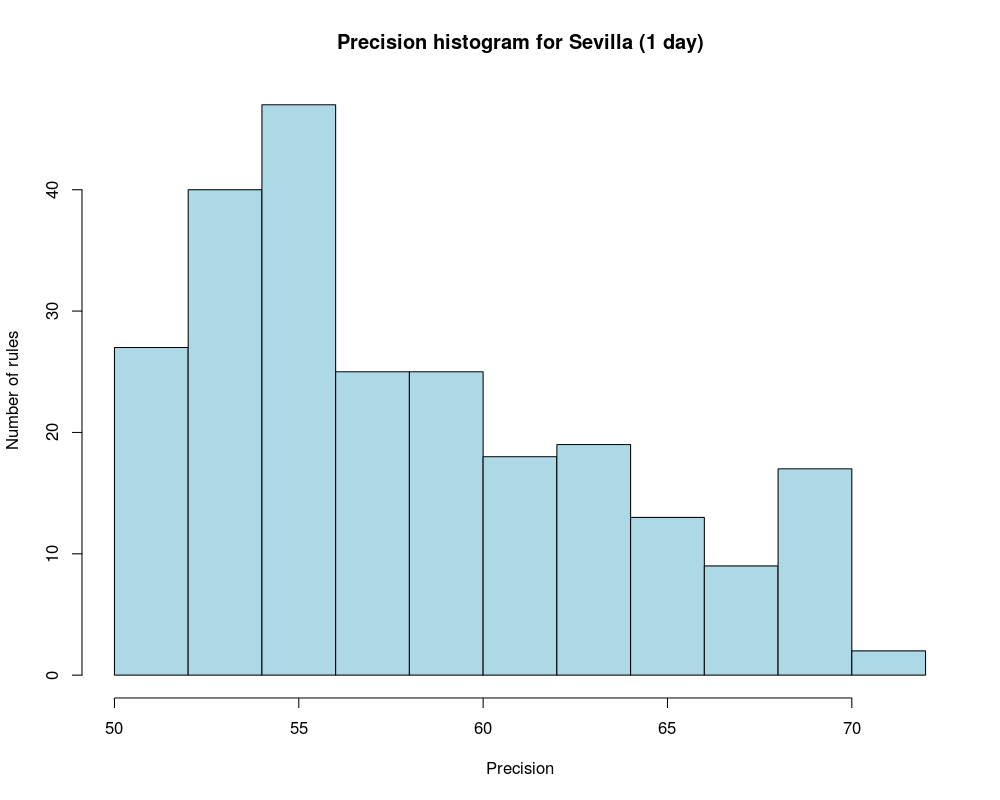
\includegraphics[width=\textwidth]{img/hist_sev1.png}
\caption{Rule distribution by precision in Station D (1 day)} \label{fig:hist_sev1}
\end{figure}

\subsection{Predictable events by category}
As we mentioned in section~\ref{sec:using_event_type}, one of the methods followed in order to being able to perform deep searches on our data was clustering by event types. This unavoidably leads to differences on the achievable performance for each of the different event types. This is caused not only by the different search depths which we were able to use in each of the different groups, but also by the individual nature of each of the event types: events in some of the clusters may be more likely to be related to others in the same cluster while for other types these relations may be more likely to be found to events in other clusters. 

In order to analyse the effect of this clustering in the obtained results, we will analyse the category of the events the rules predict. This is, we will analyse the event type of the consequent of our rules. This distribution can be seen in figures \ref{fig:conseqtypes_alb7}, \ref{fig:conseqtypes_ant1}, \ref{fig:conseqtypes_seg1}, \ref{fig:conseqtypes_seg2}, \ref{fig:conseqtypes_seg7} and \ref{fig:conseqtypes_sev1}.

We can see a completely uneven distribution in terms of rule generation for each event type. This is likely to be caused by two facts: nature of the events themselves (how unpredictable or related to other events they are) and frequency adequation (events which happen too often instead of only in specific situations might be harder to predict). Also, the different limit on search depth we were able to impose for the different groups also vastly affects results in this direction.

It is specially interesting the situation in \emph{Station B}, where we performed an alternative clustering method as mentioned in \ref{sec:group_elements}. In this station, we observe that all the rules fall into the category of \emph{Type 3} and \emph{Type 7}. Both groups of rules are quite similar in size, although the occurence of those alarm types in the whole database is significantly different. This indicates that this kind of clustering might significantly help in order to obtain more uniform results for all the event types.

\begin{figure}[hbtp]
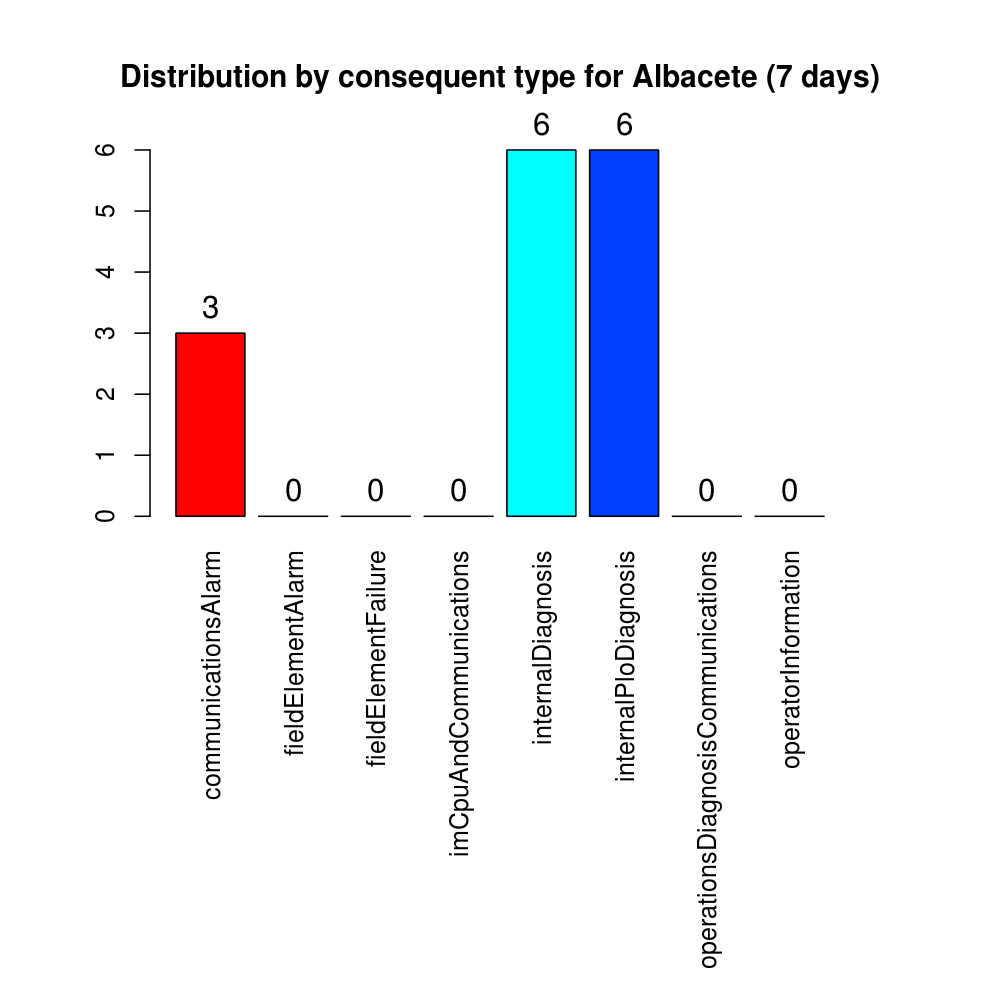
\includegraphics[width=\textwidth]{img/conseqtypes_alb7.png}
\caption{Rule distribution by consequent type in Station A (7 days)} \label{fig:conseqtypes_alb7}
\end{figure}

\begin{figure}[hbtp]
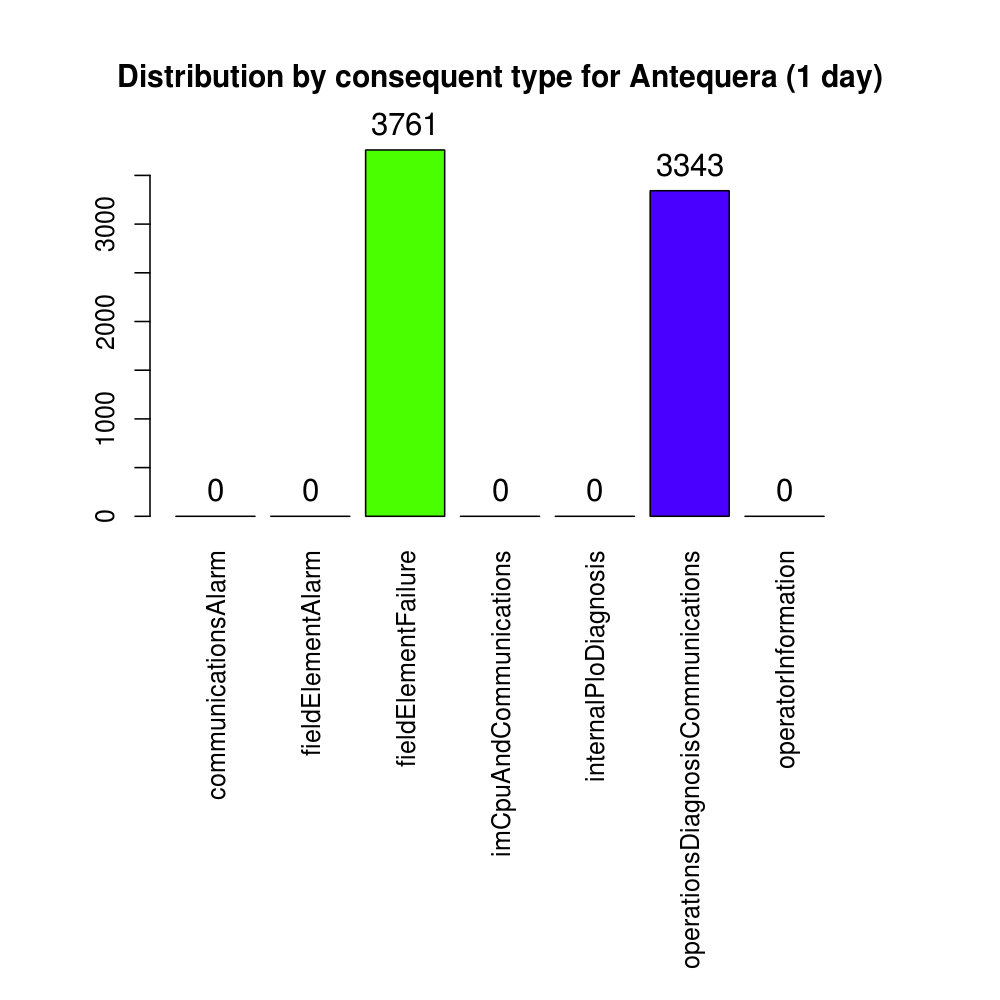
\includegraphics[width=\textwidth]{img/conseqtypes_ant1.png}
\caption{Rule distribution by consequent type in Station B (1 day)} \label{fig:conseqtypes_ant1}
\end{figure}

\begin{figure}[hbtp]
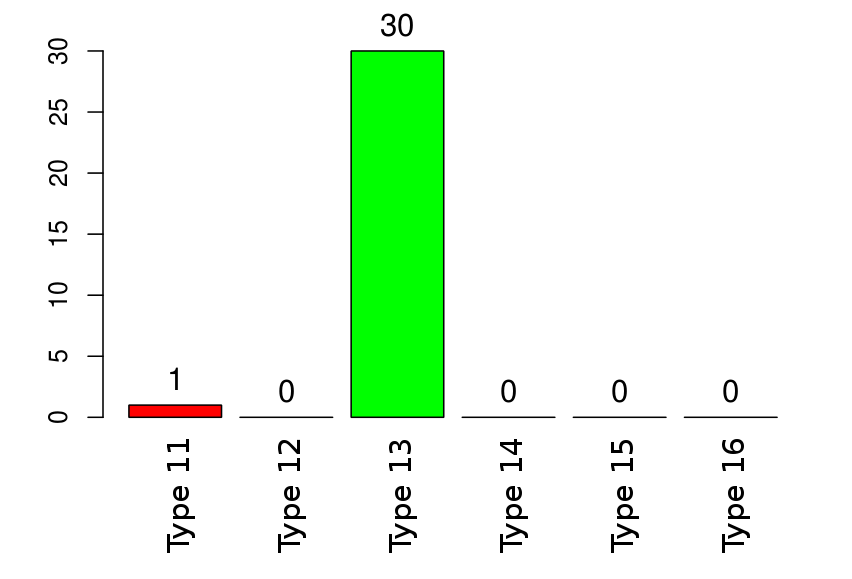
\includegraphics[width=\textwidth]{img/conseqtypes_seg1.png}
\caption{Rule distribution by consequent type in Station C (1 day)} \label{fig:conseqtypes_seg1}
\end{figure}

\begin{figure}[hbtp]
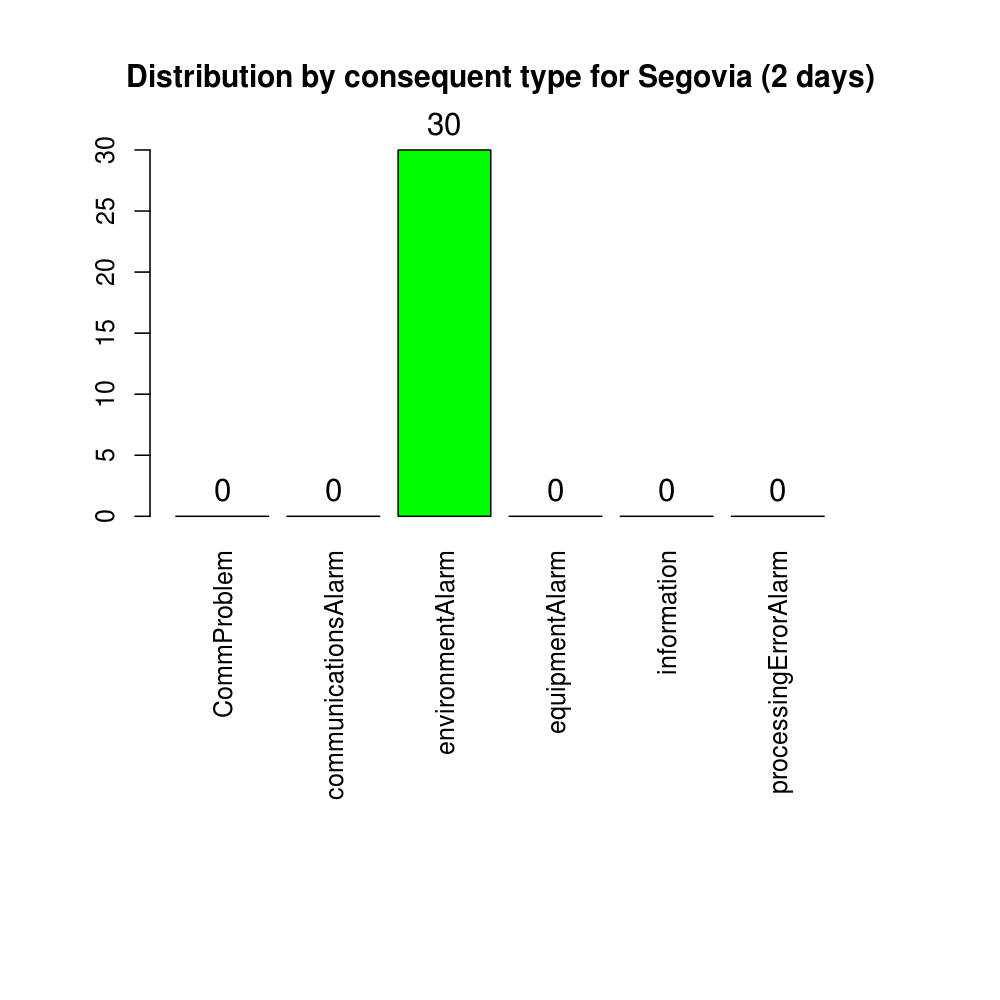
\includegraphics[width=\textwidth]{img/conseqtypes_seg2.png}
\caption{Rule distribution by consequent type in Station C (2 days)} \label{fig:conseqtypes_seg2}
\end{figure}

\begin{figure}[hbtp]
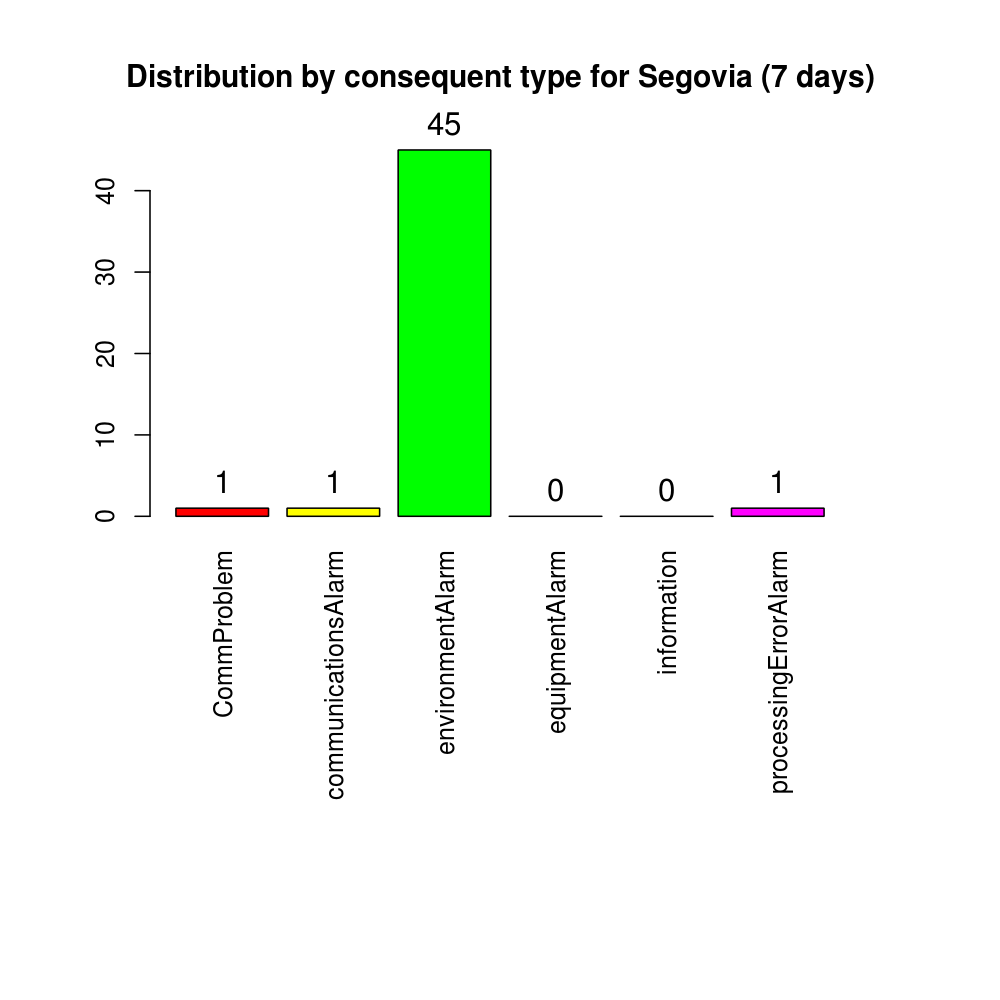
\includegraphics[width=\textwidth]{img/conseqtypes_seg7.png}
\caption{Rule distribution by consequent type in Station C (7 days)} \label{fig:conseqtypes_seg7}
\end{figure}

\begin{figure}[hbtp]
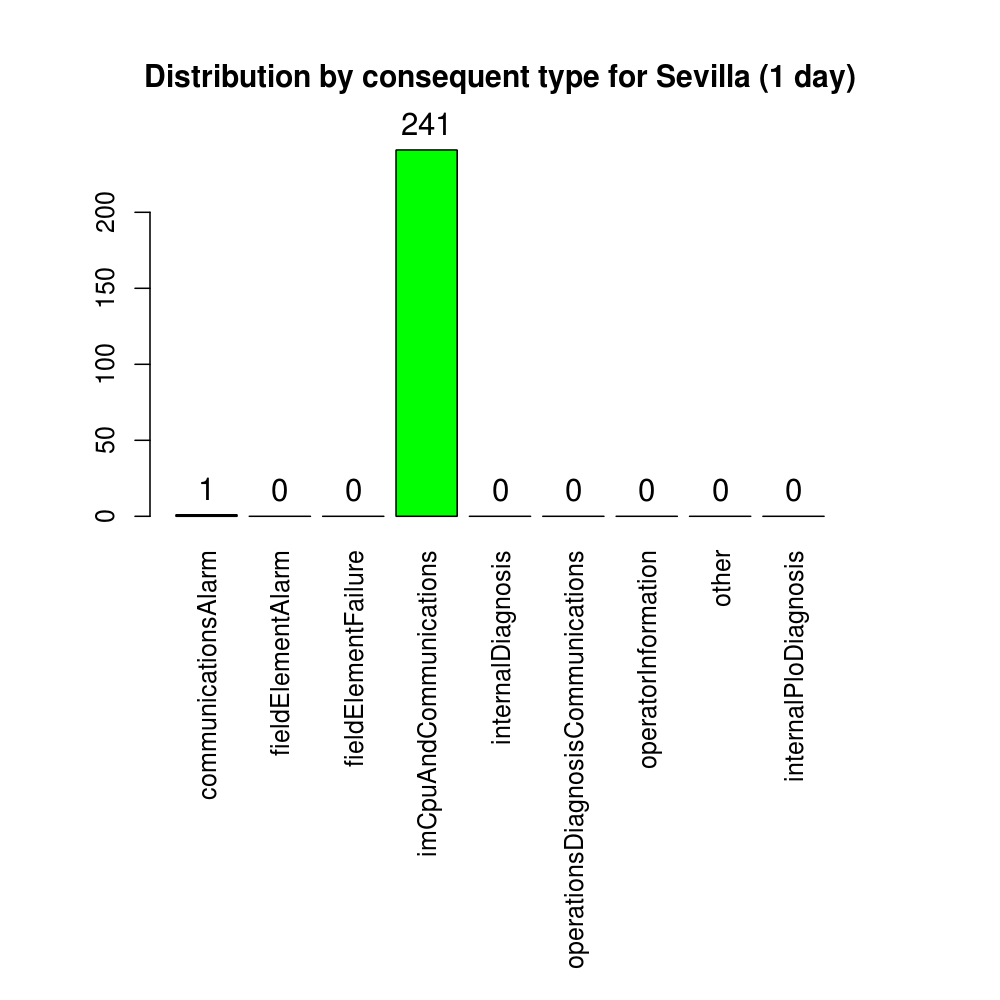
\includegraphics[width=\textwidth]{img/conseqtypes_sev1.png}
\caption{Rule distribution by consequent type in Station D (1 day)} \label{fig:conseqtypes_sev1}
\end{figure}


\section{Example scenario}
\label{sec:scenario}

In this section we will analyse the output of our predictive model during a short period of time. We will illustrate the kind of information an operator could obtain from an average period of time. Specifically, we will take a random period of 50 consecutive days for the \emph{Station B}, over which we will perform predictions for the next days.

It is important to note that this example scenario has been obtained using the rule set with precisions higher than 0.50. In a real scenario, an operator could select a higher threshold for predictions or disregard those raised predictions with a low confidence.

\subsection{Predictions raised by event type}
First of all we will observe the number of predictions raised each day of our sample. This will give us an idea of the number of predictions our system would give for an average day. This can be seen in figure~\ref{fig:scenario_pred_categories}.

As we can see, for this station and rule set the number of predictions obtained in an average day is around 20. This does not include repeated predictions (more than one rule which can be fired simultaneously to predict the same event with different confidences).

\begin{figure}[hbtp]
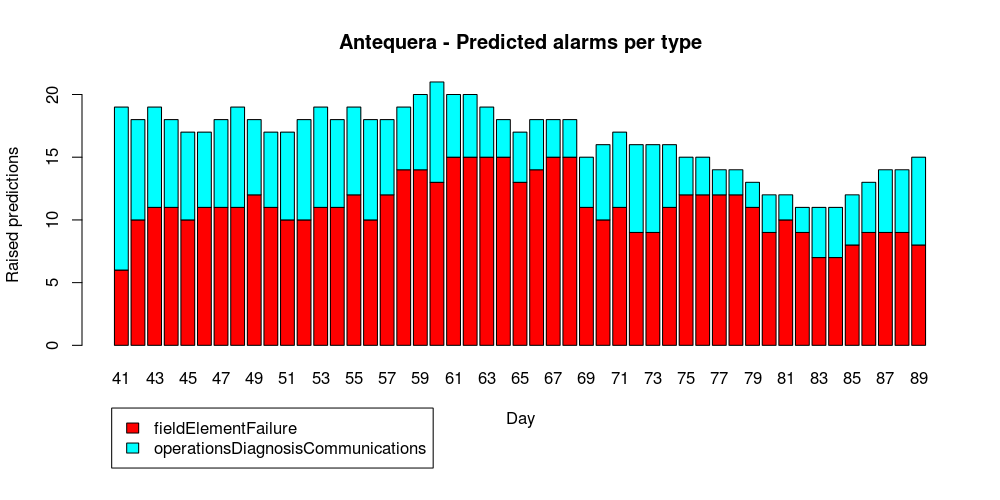
\includegraphics[width=\textwidth]{img/scenario_pred_categories.png}
\caption{Timeline of predictions during a sample period} \label{fig:scenario_pred_categories}
\end{figure}

\subsection{Percentage of events predicted}
The next thing we can analyse is the number of events which happen during an average day which are actually predicted by our system. The result is illustrated in figure~\ref{fig:scenario_pred_notpred}. This value corresponds with what we defined as \emph{recall} in section~\ref{sec:validation_evaluation}.

\begin{figure}[hbtp]
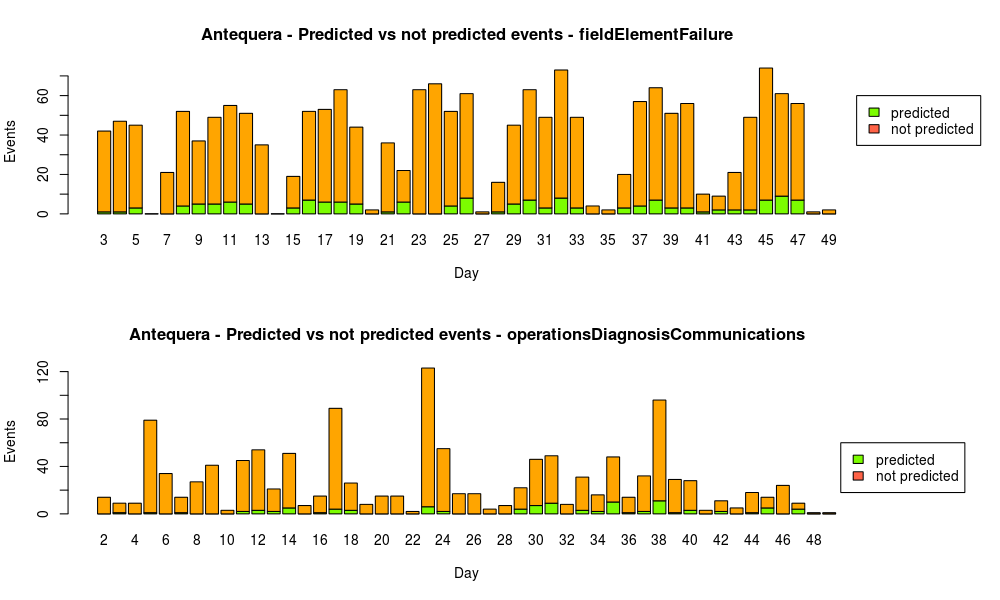
\includegraphics[width=\textwidth]{img/scenario_pred_notpred.png}
\caption{Timeline of predictions during a sample period} \label{fig:scenario_pred_notpred}
\end{figure}

\subsection{Percentage of right predictions}
To end with, we will analyse how many of the raised predictions are actually true. In order to illustrate better this aspect and take into account also the confidence parameter of the predictions, we will perform three different analysis: one disregarding predictions with $c < 0.5$, a second one with $c < 0.7$ and a third with $c < 0.8$. The results can be seen in figures \ref{fig:scenario_right_wrong}, \ref{fig:scenario_right_wrong_70} and \ref{fig:scenario_right_wrong_80} respectively.

As expected, when increasing the precision threshold we have less and less predictions, but these tend to be more accurate.

\begin{figure}[hbtp]
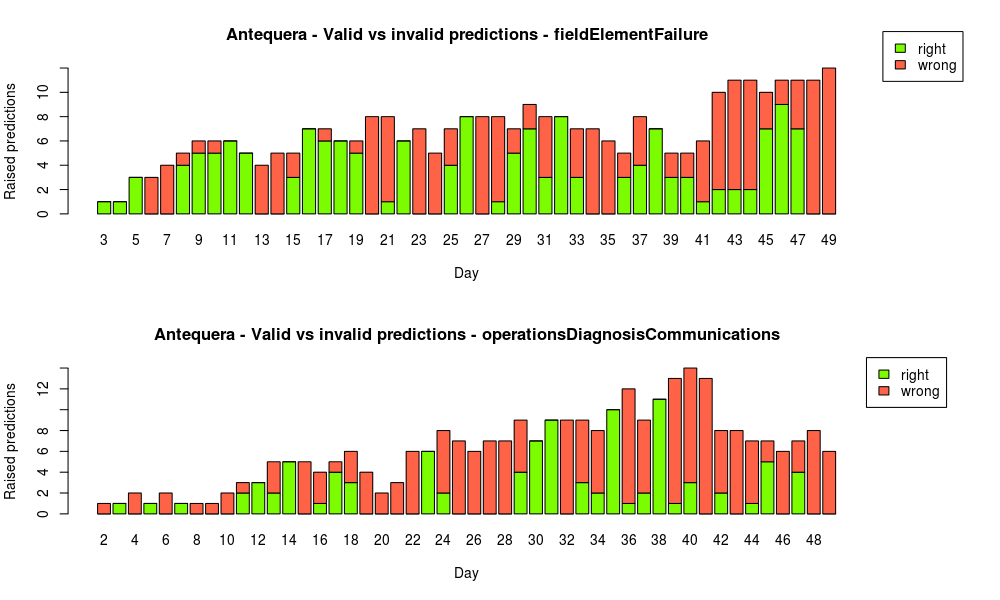
\includegraphics[width=\textwidth]{img/scenario_right_wrong.png}
\caption{Timeline of predictions during a sample period} \label{fig:scenario_right_wrong}
\end{figure}

\begin{figure}[hbtp]
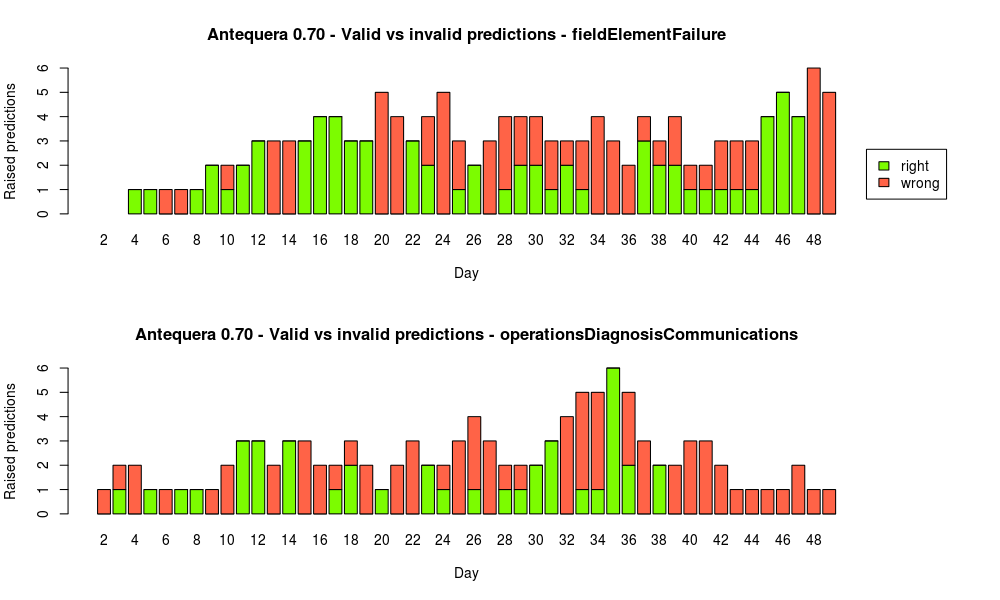
\includegraphics[width=\textwidth]{img/scenario_right_wrong_70.png}
\caption{Timeline of predictions during a sample period} \label{fig:scenario_right_wrong_70}
\end{figure}

\begin{figure}[hbtp]
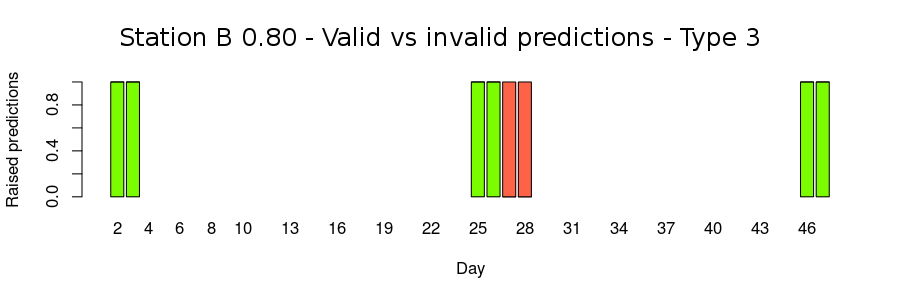
\includegraphics[width=\textwidth]{img/scenario_right_wrong_80.png}
\caption{Timeline of predictions during a sample period} \label{fig:scenario_right_wrong_80}
\end{figure}

\clearpage

\section{Conclusions}
The results obtained after the development of the presented procedures are found to be satisfactory, as shown in section~\ref{sec:desc_results}. Large rule sets with high precision values have been found for several stations and different time windows.

For this rulesets to be useful for Thales' operators, a implementation of a rule engine is necessary. This aspect with be covered in next stages of the project, and it is completely independent from the procedures described in this document which were used to obtain the predictive knowledge.

Also, results have been found to vary significantly in terms of quantity and precision in different stations and time periods, as seen in section~\ref{sec:desc_results}. In order to obtain higher quality results, it is necessary to explore alternative methods which can get over the limitations found with the performed method. First of all, the used algorithms can be vastly optimised to perform much better in our specific scenario. When searching for frequent sequences, we cannot limit the number of terms in the \emph{consequent}, as the maximum number of terms in each member of the sequence is fixed by a single parameter. In our case, we do not want to use sequences with more than one element in the consequent (as explained in section~\ref{sec:rule_model}) but our algorithm is still generating them as sequence candidates. This increases the complexity of the algorithm significantly, as we are growing our candidates in both the antecedent and the consequent of the rule while we only need the antecedent to 
grow.

Furthermore, as mentioned in section~\ref{sec:rule_model}, the candidates for rules are selected amongst sequences which are \emph{frequent}. Although this provides a good starting point in order to find predictive rules, we must perform two kinds of filtering in order to obtain the final rule sets: first by frequency, and later by precision. A new algorithm could be implemented in the same fashion as cSPADE, but performing only a filtering in terms of precision. This would not only save time and allow deeper searches, but also avoid disregarding those sequences which are not frequent but might lead to precise predictions.

Additionally, as seen in chapter~\ref{chap:datamining}, there are many other types of data mining algorithms which could be used or adapted to our problem. Specifically, a parallell approach has been made using \emph{Bayesian Networks}. These networks provide a very useful mathematical model which can be used to predict information in a similar fashion than the rules. However, it usually requires a deep previous knowledge on the events of the system and their possible relations in order to obtain their full potential. After building some of these models and obtaining said information from Thales' engineers, the model based on \emph{association rules} was still found to perform much better in all terms. Additional research would be necessary in order to obtain better results with these alternative tools.

Finally, we have found that one of the best and most immediate ways to increase the quality of the results is to divide the large datasets into smaller clusters. In section~\ref{sec:dataclustering} we have presented two possible clustering methods which have indeed improved the results significantly. Further improvement could be achieved by performing a deeper research on alternative clustering methods. Specifically, the method described in section~\ref{sec:group_elements} was found to increase peformance in very high rates. Developing a way to make this clustering method automatisable and directly feasible for all the stations would likely highly increase performance.

Summarising, in order to obtain higher quality results, a way must be found to face limits in terms of computation capabilities. The server available for our project is powerful enough as to think of improving hardware. Therefore, software and data optimisation is the only way to obtain significant improvement in the results.